\documentclass{article}

\usepackage[utf8]{inputenc}
\usepackage[english]{babel}
\usepackage{biblatex}
\addbibresource{proposal.bib}
\usepackage[colorinlistoftodos]{todonotes}
\usepackage{graphicx}
\graphicspath{{./figures/}}
\usepackage{tikz}
\usepackage{amsmath}
\usepackage{csquotes}

\title{Applications of Neural Networks to Solve the Differential Equations of Magnetohydrodynamics}

\author{Ph.D. Thesis Proposal\\Eric Winter\\George Mason University\\Department of Physics and Astronomy}

%%%%%%%%%%%%%%%%%%%%%%%%%%%%%%%%%%%%%%%%%%%%%%%%%%%%%%%%%%%%%%%%%%%%%%%%%%%%%%%%

\begin{document}

\begin{titlepage}
\maketitle
\end{titlepage}

%%%%%%%%%%%%%%%%%%%%%%%%%%%%%%%%%%%%%%%%%%%%%%%%%%%%%%%%%%%%%%%%%%%%%%%%%%%%%%%%

\begin{abstract}

The proposed work will provide a novel capability for efficiently solving the equations of magnetohydrodynamics (MHD) for space plasma scenarios. Previous work has shown the efficacy of using neural networks with one or more hidden layers to solve simple ordinary and partial differential equations, but these techniques will be extended to create the first neural network-based solution of the coupled set of 2nd-order partial differential equations which describe MHD in space. Several distinct MHD regimes will be examined. The technique will be applied first to relatively simple model scenarios, such as the steady-state solar wind flow, and the propagation of magnetic flux lines from the solar photosphere to the corona. Then the mechanism will be extended to more complex scenarios with dynamic boundary conditions, such as coronal mass ejections, and the onset and propagation of plasma wave phenomena. These techniques will provide a set of solutions that are completely mesh-free, and differentiable. In many situations, we expect the neural network approach will prove to be significantly faster than the currently-standard techniques of the finite difference method (FDM) and the finite element method (FEM). The neural network method will be shown to be more efficient in its use of computational resources, and provide a solution which is at least as accurate as solutions from traditional methods. This work will provide a critical, independent solution of the MHD equations, which can be used in conjunction with existing heritage models to improve the speed and accuracy of analyses of space plasma and space weather events.

\end{abstract}

%%%%%%%%%%%%%%%%%%%%%%%%%%%%%%%%%%%%%%%%%%%%%%%%%%%%%%%%%%%%%%%%%%%%%%%%%%%%%%%%

\newpage

\tableofcontents

%%%%%%%%%%%%%%%%%%%%%%%%%%%%%%%%%%%%%%%%%%%%%%%%%%%%%%%%%%%%%%%%%%%%%%%%%%%%%%%%

\newpage

\section{Overview}

\subsection{Scientific Rationale}

The differential equations of magnetohydrodynamics (MHD) govern the behavior of all space plasmas, and thus are the primary equations which govern the behavior of space weather phenomena. As our reliance on space-based assets for communication, observation, and exploration has increased, the vulnerability of those assets to severe space weather events has also increased \cite{NRC2009}. If the speed and accuracy of models of space weather events can be improved, the risk to personnel and material assets in space can be reduced by providing increased warning time, allowing improved preparations to withstand the potential consequences of the event.

The MHD equations combine the mechanics of fluid flow with Maxwell's equations of electrodynamics. Similar to the Navier-Stokes equations, the MHD equations describe the effects of the conservation of mass, momentum, and energy. But the MHD equations also account for the conservation of electric charge and magnetic flux, and the interdependence of charges, currents, electric, and magnetic fields. The detailed form of the equations is dependent on the assumptions made in their derivation. For example, for flow of an ideal, adiabatic, shock-free plasma, with a single ion species (the ``single-fluid" case), the MHD equations \cite{Chen1984} become:

\bigskip

Gauss' Law
\begin{equation}
    \epsilon_0 \nabla \cdotp \mathbf E = n_i q_i + n_e q_e
    \label{eq:GaussLaw}
\end{equation}

Faraday's Law
\begin{equation}
    \nabla \times \mathbf E = -\frac {\partial \mathbf B} {\partial t}
    \label{eq:FaradayLaw}
\end{equation}

Magnetic divergence (no magnetic monopoles)
\begin{equation}
  \nabla \cdotp \mathbf B = 0
  \label{eq:mhd_MagneticDivergence}
\end{equation}

Amp\`{e}re's Law
\begin{equation}
    \frac {1} {\mu_0} \nabla \times \mathbf B = n_i q_i \mathbf v_i + n_e q_e \mathbf v_e + \epsilon_0 \frac {\partial \mathbf E} {\partial t}
    \label{eq:AmpereLaw}
\end{equation}

Conservation of mass ($j = i|e$)
\begin{equation}
    \frac {\partial n_j} {\partial t} + \nabla \cdotp \left(n_j \mathbf v_j \right) = 0
    \label{eq:ConservationOfMass}
\end{equation}

Conservation of momentum ($j = i|e$)
\begin{equation}
  m_j n_j \left[ \frac {\partial \mathbf v_j} {\partial t} + \left( \mathbf v_j \cdotp \nabla \right) \mathbf v_j \right] = q_j n_j \left(\mathbf E + \mathbf v_j \times \mathbf B \right) - \nabla P_j - m_j n_j \nu_{jn} \mathbf v_j
  \label{eq:ConservationOfMomentum}
\end{equation}

Pressure gradient ($j = i|e$)
\begin{equation}
    \nabla P_j = \gamma_j k T_j \nabla n_j
    \label{eq:PressureGradient}
\end{equation}

\noindent However, (\ref{eq:GaussLaw}) and (\ref{eq:mhd_MagneticDivergence}) are superfluous, since they can be obtained from the divergence of (\ref{eq:AmpereLaw}) and (\ref{eq:FaradayLaw}), respectively. We close this system of equations by assuming an adiabatic plasma, so a solution is possible, in principle. This solution incorporates the effects of the electric and magnetic fields on plasma motion, and the effects of plasma motion on the electric and magnetic fields, in a self-consistent manner.

These equations can be used as the starting point for the investigation of specific plasma environments and phenomena. For example, space plasmas can usually be treated as collisionless and adiabatic, and (\ref{eq:ConservationOfMomentum}) becomes:

\begin{equation}
    \mathbf E + \mathbf v_j \times \mathbf B = 0
    \label{eq:IdealMHDOhmLaw}
\end{equation}

\noindent This result leads to the ``frozen-in" condition, in which the magnetic flux is essentially carried along by the flowing plasma. The magnetic field of the solar plasma is one of the primary inputs for models of space weather phenomena in the vicinity of planetary magnetospheres. For example, when the solar and terrestrial fields are roughly anti-parallel, magnetic field reconnection events can become more frequent and more powerful, leading to solar storms and substorms.

The MHD equations can be used to model regions progressively more distant from the Sun. For example, a simpliified two-dimensional MHD model can be used to examine the evolution of active region magnetic fields in the solar photosphere \cite{russell2016}. In this case, the analysis occurs on a two-dimensional surface in spherical coordinates (\ref{eq:PhotosphereField}).

\begin{equation}
\begin{split}
    \frac {\partial B_r} {\partial t} + \frac {1} {R_S \sin \theta} \frac {\partial} {\partial \theta} \left( v_{\phi} B_r \sin \theta \right) + v_{\theta} \frac {\partial B_r} {\partial \phi} \\
    + \frac {\eta} {R_S^2 \sin \theta} \frac {\partial} {\partial \theta} \left( \sin \theta \frac {\partial B_r} {\partial \theta} \right) + \frac {\eta} {R_S^2 \sin^2 \theta} \frac {\partial^2 B_r} {\partial \phi^2} = S(\theta, \phi, t)
    \label{eq:PhotosphereField}
\end{split}
\end{equation}

\noindent where $\eta$ is the diffusivity, and $S$ is a source term representing the creation of new active regions. This equation can be used to model the evolution of the photospheric magnetic field represented by solar synoptic maps.

Moving further outward, the connection between the surface field and the coronal field can be modeled with the potential field source surface (PFSS) model \cite{Altschuler1969}. The PFSS model is a conceptually simple model used to estimate the solar coronal magnetic field from observations of the surface magnetic field. In this model, the static coronal field is derived from a scalar magnetic potential field:

\begin{align}
    \mathbf B &= - \nabla \phi \\
    \nabla^2 \phi &= 0 \\
    B_r &= - \frac {\partial \phi} {\partial r} \\
    B_{\theta} &= - \frac {1} {r} \frac {\partial \phi} {\partial \theta} \\
    B_{\phi} &= - \frac {1} {r \sin \theta} \frac {\partial \phi} {\partial \phi}
    \label{eq:PFSS}
\end{align}

\noindent Despite its greatly simplified structure, the PFSS has proven so useful that it is included in the catalog of standard models offered by the Community Coordinated Modeling Center (see discussion of the CCMC below).

A more rigorous model of the coronal magnetic field, developed by \cite{Endeve2003}, provides additional levels of detail in the model, including predictions of regions of trapped plasma, and the high-latitude "last closed field lines":

\bigskip

Conservation of mass
\begin{equation}
    \frac {\partial \rho} {\partial t} + \nabla \cdotp \left(\rho \mathbf u \right) = 0
    \label{eq:ELH1}
\end{equation}

Conservation of momentum
\begin{equation}
    \frac {\partial \left( \rho \mathbf u \right)} {\partial t} + \nabla \cdotp \left(\rho u \mathbf u \right) = - \nabla P - \frac {G M_S} {r^2} \rho \mathbf {\hat r} + \mathbf j \times \mathbf B
    \label{eq:ELH2}
\end{equation}

Amp\`ere's Law
\begin{equation}
    \mathbf j = \frac {1} {\mu_0} \nabla \times \mathbf B
    \label{eq:ELH3}
\end{equation}

Magnetic induction
\begin{equation}
    \frac {\partial B} {\partial t} = \nabla \times \left( \mathbf u \times \mathbf B \right)
    \label{eq:ELH4}
\end{equation}

Ideal gas law
\begin{equation}
    P = \frac {n k T} {m}
    \label{eq:ELH5}
\end{equation}

Beyond the corona, the solar atmosphere merges into the solar wind. The solar wind is typically modeled as a high-speed collisionless plasma with a frozen-in magnetic field. Various forms of the MHD equations are implemented in a variety of models used to analyze the solar wind. Models used for day-to-day space weather monitoring and prediction typically have a longer heritage than research models. For example, the NOAA Space Weather Prediction Center \cite{swpc} maintains a stable of operational models and a large archive of historical data of solar activity and space weather. These products are used to produce short-term (3-day) and long-term (27-day) forecasts of solar activity and space weather conditions, which are also used as the basis for geomagnetic storm and other space weather warnings.

An example of these models is the WSA-ENLIL combined model \cite{wsaenlil}. This model has been used operationally at the NOAA SWPC since 2011. It is a semi-empirical model that predicts the speed, density, temperature, magnetic field, and other parameters of the “ambient” (non-CME) solar wind at 1 AU, and is thus a useful predictive tool for terrestrial space weather events. This model was deployed because full three-dimensional MHD simulations still take too much time to set up, run, and validate. The modeling system consists of two main parts: (1)  a semi-empirical near-Sun module (WSA - Wang-Sheeley-Arge \cite{Arge2000},\cite{Sheeley2017}) that approximates the outflow at the base of the solar wind; and (2) ENLIL \cite{enlil}, a sophisticated three-dimensional magnetohydrodynamic numerical model that simulates the resulting flow  evolution out to 1 AU. In addition to the SWPC, a wide variety of modern and legacy research models are available at the NASA Community Coordinated Modeling Center (CCMC) \cite{ccmc} at the NASA Goddard Space Flight Center. The results of these models are made available with scheduled and on-demand runs for the community, as well as an extensive archive.

\subsection{Solving Differential Equations}

The MHD equations (in any form) constitute a set of coupled partial differential equations (PDEs) that are second-order in spatial variables and first-order in time. Additionally, since these equations arise from conservation laws, the partial differential equations themselves are \textit{hyperbolic}. Hyperbolic equations result in solutions with propagating behavior - a wave equation is a typical case. Solutions may be found using any of the current standard techniques for PDEs. Chief among these are the finite difference method (FDM) and the finite element method (FEM).

In the finite difference method \cite{Heath2002}, derivatives of the function field are approximated by difference equations using Taylor series. The difference equations are defined at a mesh of grid points in the problem domain. The result is a system of linear algebraic equations that must be solved to generate the solution at the selected grid points. The solution at non-grid points must be estimated using an interpolation scheme, or computing a new solution with a new grid. Finite difference methods have the advantage of conceptual simplicity and well-developed computational techniques. However, finite difference methods can be inefficient in situations where boundary conditions or physical parameters are dynamic, since any change requires a new solution of the entire set of coupled difference equations. Additionally, parallelization of the FDM can be a complex endeavor, since each mesh element depends on its neighboring elements. To avoid saturation of the parallel computing system, the domain mesh must be carefully partitioned among the available computation threads to minimize inter-thread communication during the solution process, e.g. \cite{Schreiber2017}.

In the finite element method \cite{DeVries2011}, the problem domain is also subdivided into a mesh, and the differential equations of the system are defined for each subvolume of the domain. The collection of equations is then used to define a global error function. This error function is then minimized by an appropriate method, and the parameter vector which minimizes the error function defines the solution to the problem. Like FDM, changes in location, system parameters, or boundary conditions require an interpolation scheme or a completely new solution cycle. FEM solutions also suffer from the same parallelization difficulties as FDM, leading to complicated code for large problems. Both FDM and FEM techniques suffer from increased approximation error as a function of time \cite{Carnahan1969}, which can lead to additional recomputations of the solutions for new boundary conditions. Adaptive mesh refinement, e.g. \cite{Berger1989}, can improve the quality of the solution in regions of rapid change, but solutions are still only available at the selected grid points. Several packages are available to address these issues, such as the widely-used PETSc toolkit \cite{petsc}, which provides support for the parallel distribution of matrices used in finite element models.

Since the late 1980s, new approaches for the solution of differential equations have been developed which take advantage of neural networks. There are a variety of techniques available, but all take advantage of one of the most mathematically useful aspects of neural networks - the ability to act as a "universal approximator" \cite{Hornik1989}. This capability was later shown to extend to approximation of the derivatives of the function \cite{Hornik1990}. The development of this field has been surveyed in recent comprehensive reviews \cite{Yadav2015,Chakraverty2017}. Neural network techniques generate mesh-free solutions which are differentiable to a useful extent, and are easily parallelized on modern multicore computers \cite{Schuessler2011}. Drawbacks can include lengthy training times, especially in cases where local minima in the error function are encountered. Such situations can exacerbate the already long training times which result from solving higher-dimensional problems - the so-called "curse of dimensionality". However, neural network techniques have shown promise in improving performance over traditional finite difference solutions of PDEs of high dimensionality (Figure \ref{fig:Avrutskiy_2020}).

\begin{figure}
  \centering
  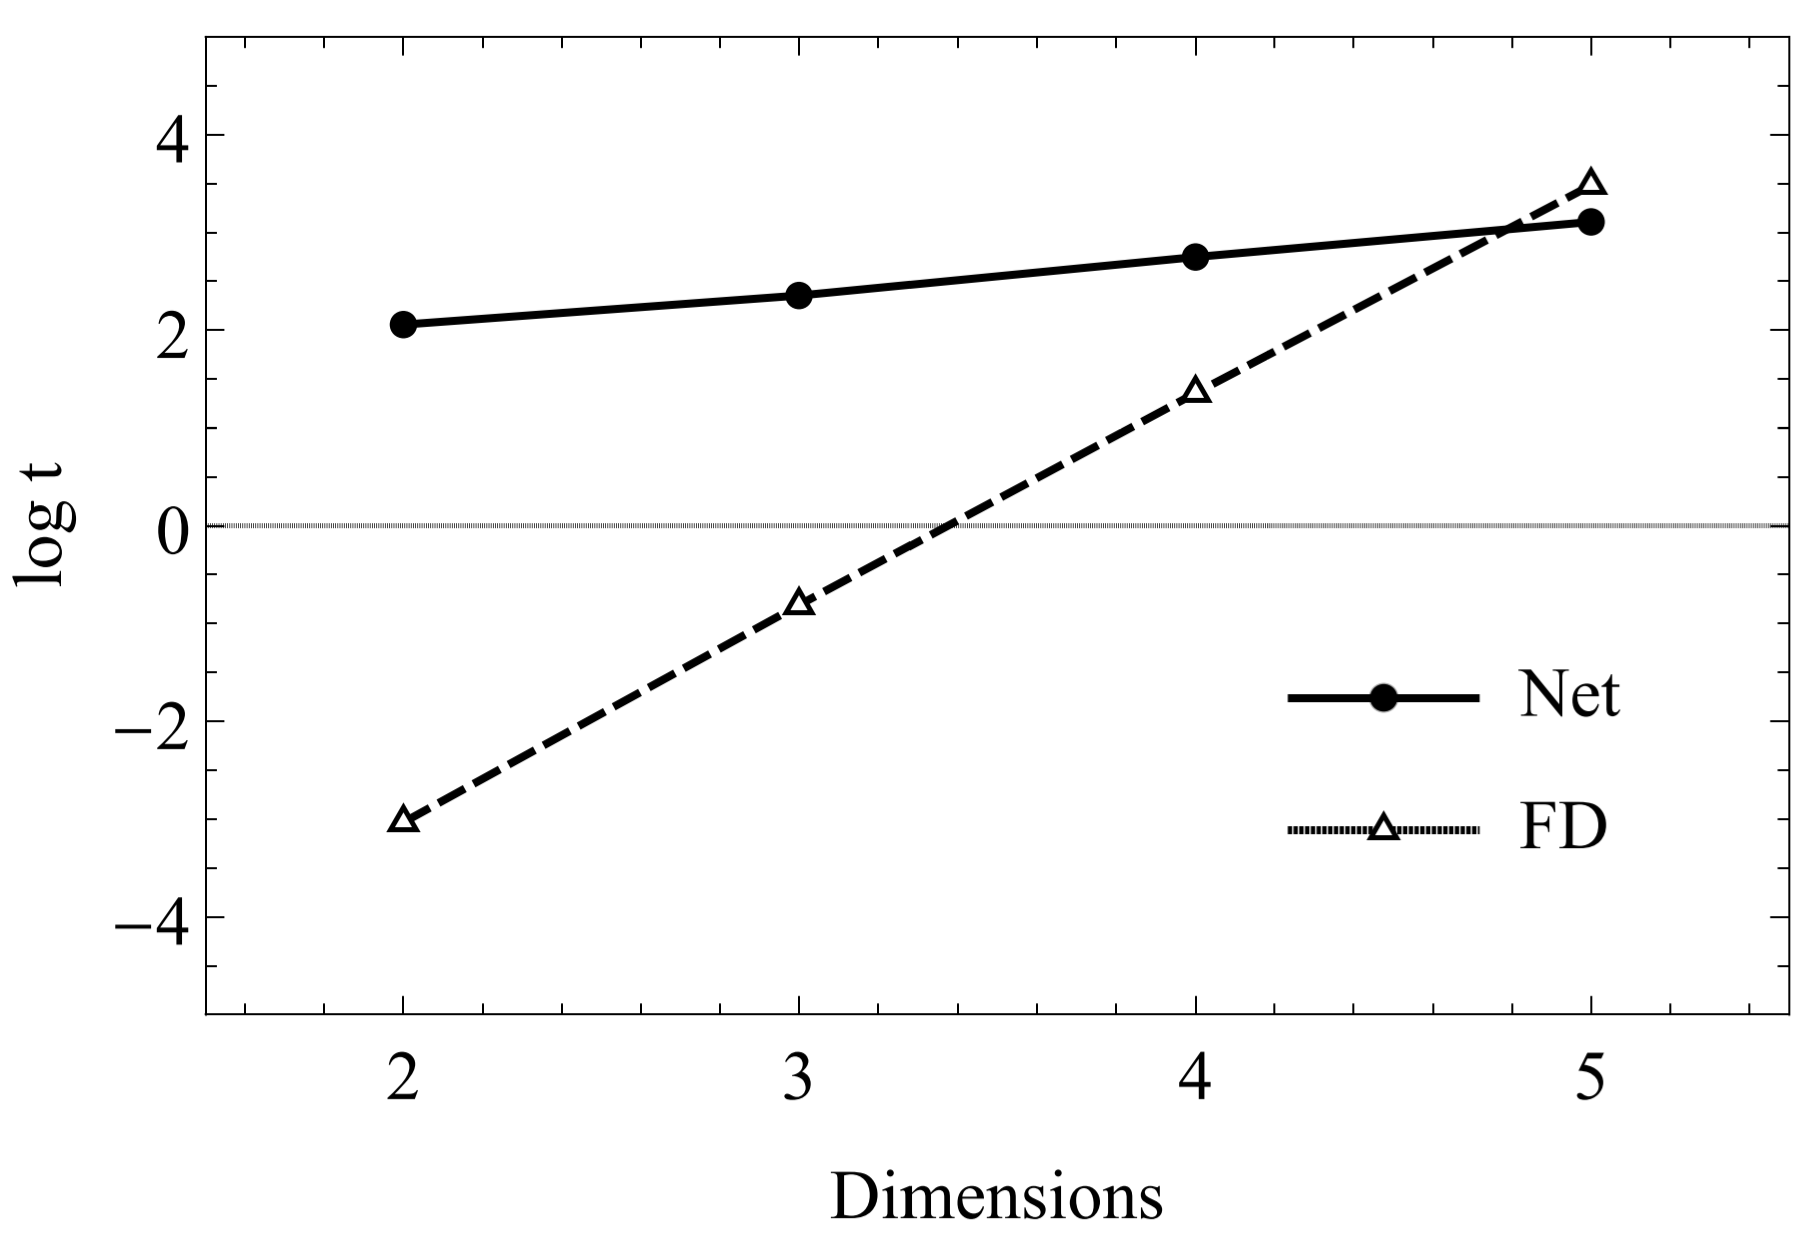
\includegraphics[width=0.75\textwidth]{Avrutskiy_2020.png}
  \caption{A comparison of solution times for neural network and 2nd-order finite difference methods for increasing problem dimensionality. The data were generated by specifying the analytical form of scalar functions of up to 5 independent variables, and substituting these solutions into linear and nonlinear forms of the Poisson equation. Training and testing points were randomly distributed on the surface of an $n$-dimensional hypersphere. Neural networks with up to 6 hidden layers were then trained to generate the solutions to compare against finite-difference solutions. Networks were trained using a GPGPU-equipped computer, and 32-bit precision. \cite{Avrutskiy2020}}
  \label{fig:Avrutskiy_2020}
\end{figure}

When the boundary conditions are dynamic, there are two basic modifications which can be made to the neural network solution. First, solutions can be generated at a representative set of times, and the solutions between those times interpolated as needed. Second, the dynamic boundary conditions themselves can be incorporated into the neural network solution itself, using either a functional or a data-based representation \cite{Lagaris1998}. The current work uses the latter approach.

\subsection{Objectives and Impact}

\subsubsection{Extend the Neural Network Computational Approach to the Coupled PDEs of MHD}

The nature of a neural network solution provides two important benefits to solving differential equations. First, since the solution is mesh-free, no interpolation or recomputation is required to generate solution values at points not used in the training process. Second, since the neural network approach provides an analytical form for the solution, the solution is easily differentiable. Previous work has claimed that the solutions are "infinitely" differentiable \cite{Lagaris1998}, and this is mathematically correct. However, experience gained during the early phases of this work have shown that the accurate differentiability extends only over a small range of orders. In the problems examined to date (typically simple second-order PDEs), the numerical values of the computed  derivatives become less accurate as the order of differentiation is increased. One of the goals of this work is to quantify the accuracy of the derivatives of the neural network solution. This investigation will provide constraints on the degree of differentiation that can be usefully applied to a neural network solution. These constraints will improve the ability to match any Neumann boundary conditions set for the problem, which will be particularly useful when estimating mass and energy fluxes at the boundaries of the problem domain.

Every increase in model computation speed will provide increased lead time to prepare for a space weather event. Neural network methods are inherently logically parallel - computations at each node are completely independent of any other node in the same layer. Neural networks are thus more easily adapted to take advantage of parallel computing hardware. This will allow rapid scaling of problem size and solution speed, as the neural network software can take advantage of both local (multi-core, multi-thread, and GPU/accelerator) and non-local (multi-node) parallelism. This capability will be particularly important for three-dimensional MHD problems, for which a large number of training points will be required.

\subsubsection{Demonstrate the Improved Utility and Efficiency of Compact Neural Network Solutions}

Current MHD models used for space plasma analysis utilize well-tested methods from FDM and FEM. However, the amount of time needed to generate the model results, as well as the storage requirements for the resulting large datasets, can limit the amount of time available to analyze the results within a useful time frame, such as an impending severe space weather event. The parameter vectors generated by the neural networks will encapsulate a compact set of solutions for the MHD equations under physically realistic conditions. These compact solutions will allow focused investigations into the specific spatial and temporal regions that are of greatest interest to the researcher.
 
The parameter vectors will be generated over a range of physical conditions, from the solar photosphere to the terrestrial magnetosphere interface. Existing standard methods, such as those discussed in the previous section, will be used as a basis for comparison for the neural network solutions. At each stage, the neural network results will be compared to equivalent results using FDM and/or FEM, to discover the parameter spaces where each method is the faster solution. The result will be a set of neural network alternative solutions for each of the space plasma regimes examined.

The software developed so far for this effort \cite{nnode} is open-source, and made available for community use on GitHub \cite{github}. Over the past two years, several experimental versions of the software for this effort have been developed. These early versions of the code have already been downloaded and/or forked several times from GitHub and used by other researchers. The rapidly-moving field of machine learning requires this approach to ensure that the latest theoretical advances are rapidly incorporated into the software.

%%%%%%%%%%%%%%%%%%%%%%%%%%%%%%%%%%%%%%%%%%%%%%%%%%%%%%%%%%%%%%%%%%%%%%%%%%%%%%%%

\newpage

\section{Background and Previous Work}

\subsection{Neural Networks}

\subsubsection{General Introduction}

The concept of computational neural networks was first introduced in the 1940s \cite{McCulloch1943}. Biological neural networks are composed of a large number of neurons, connected by axons and dendrites (Figure \ref{fig:BioNN}). Dendrites bring signals to the neuron, where they are processed as a group to generate a single output, which is then transmitted to  one or more subsequent neurons by the (often branching) axon.

\begin{figure}
  \centering
  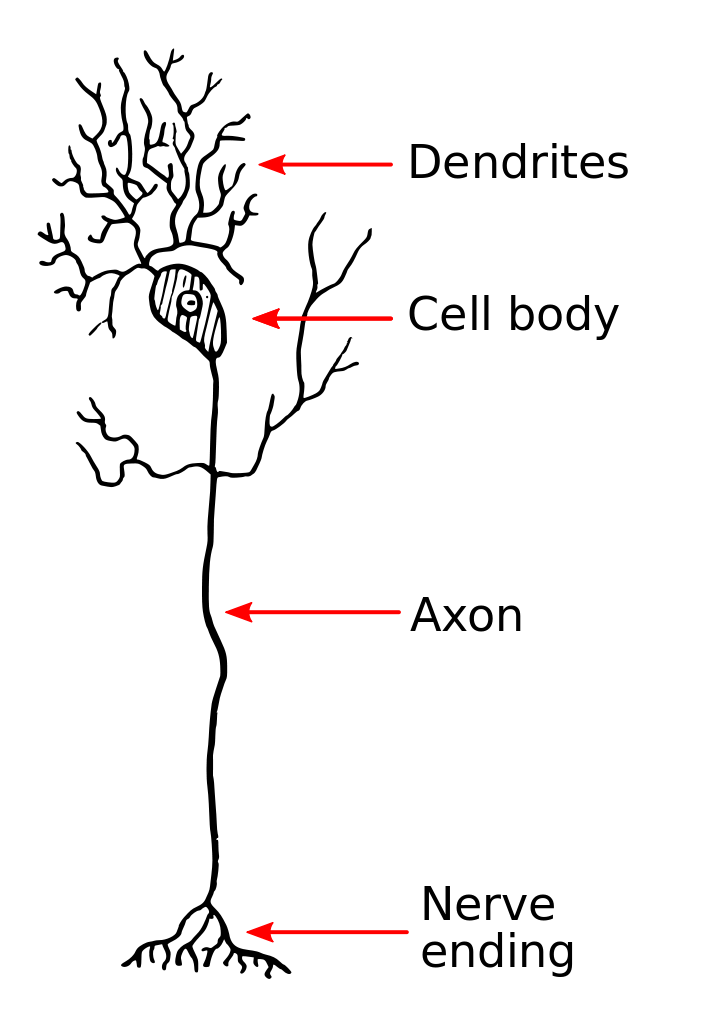
\includegraphics[width=0.5\textwidth]{Dendrite.png}
  \caption{The components of a biological neural network \cite{bionn}.}
  \label{fig:BioNN}
\end{figure}

\begin{figure}
  \centering
  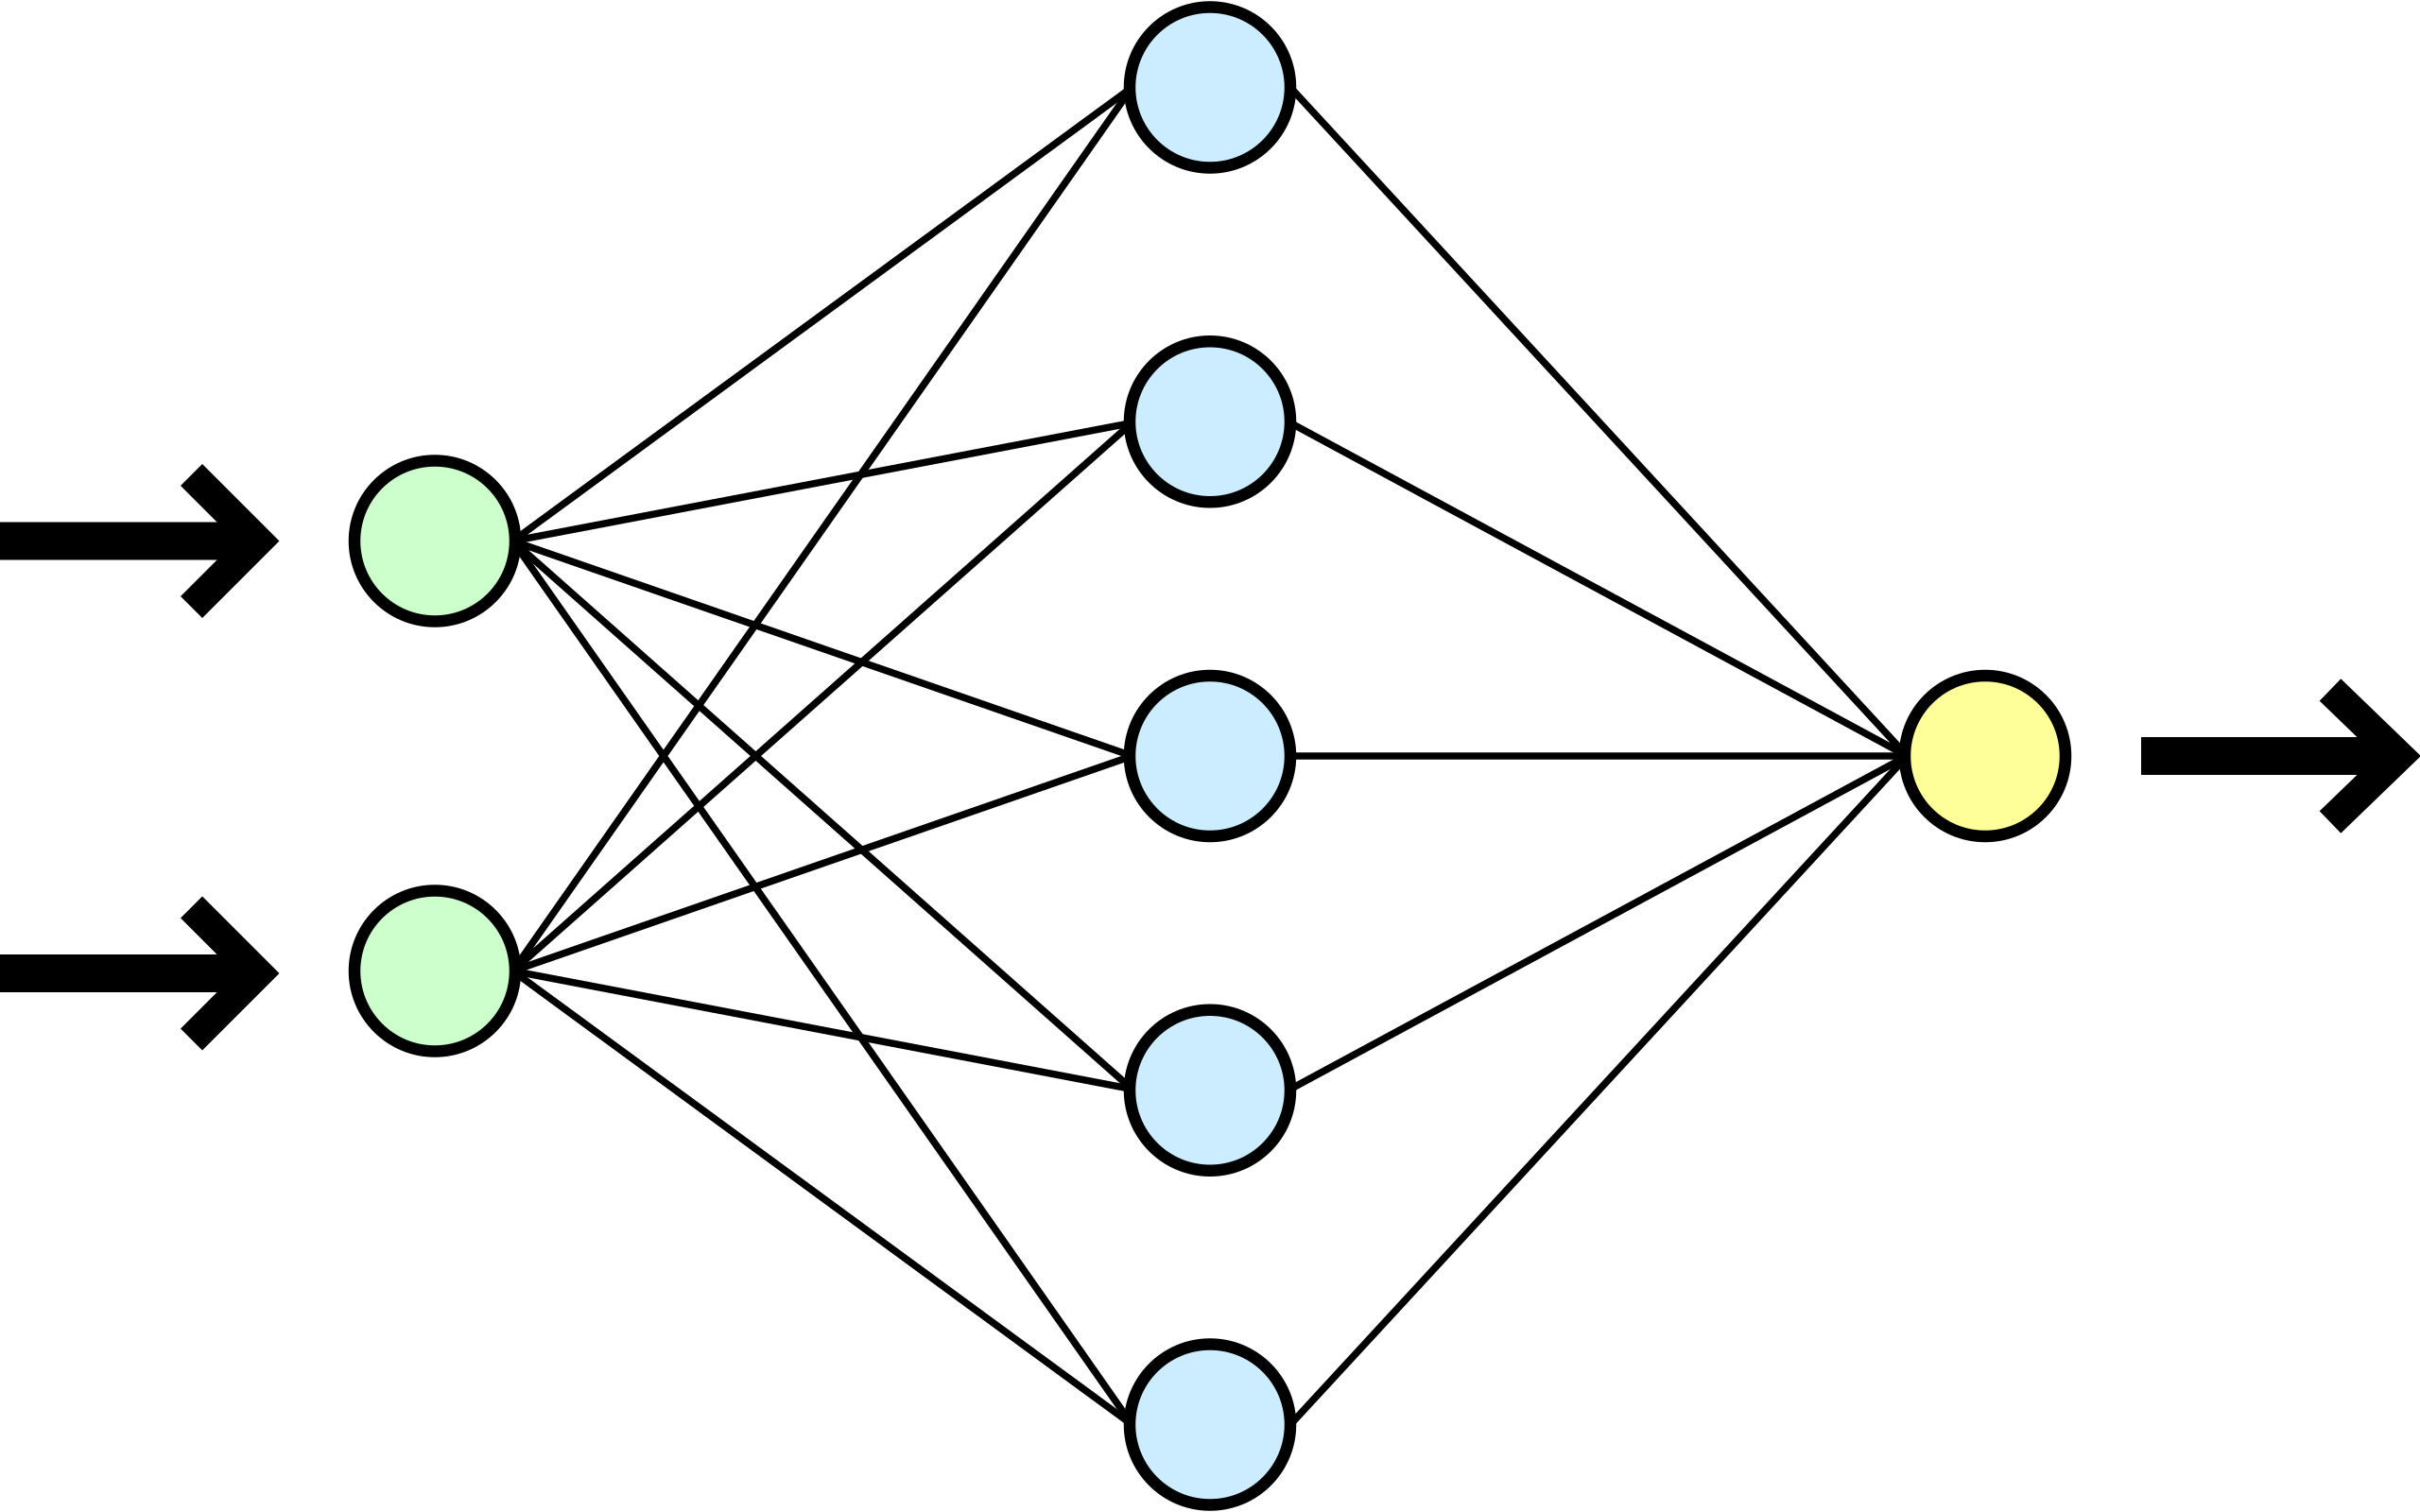
\includegraphics[width=0.5\textwidth]{NeuralNetwork.png}
  \caption{The components of a computational neural network \cite{compnn}.}
  \label{fig:CompNN}
\end{figure}

A single computational neural network node is analogous to a biological neuron, in that it receives a fixed number of inputs, and computes a weighted combination $z$ (the \emph{activation}) of the inputs $x$ (Figure \ref{fig:CompNN}). The node then applies a transfer function $\sigma(z)$ to the activation to compute a single output. This output is then transmitted to one or more subsequent nodes for further processing. The simplest version of this process can be represented as a weighted sum $z_k$ of inputs $x_j$, followed by a binary comparison to a threshold value $\theta_k$ (\ref{eq:threshholdtf}).

\begin{equation}
\begin{split}
  z_k &= \sum_{j=1}^m w_{jk} x_j \\
  \sigma(z_k) &= (z_k \ge \theta_k)\ ?\ 1:0
\end{split}
\label{eq:threshholdtf}
\end{equation}

\noindent where $j$ is an index over the $m$ inputs, and $k$ is an index over the $H$ network nodes. In this simple model, if the input exceeds a threshold value $\theta_k$, the node "fires", sending its output (unity) to subsequent nodes.

While conceptually simple, and useful in discrete classification problems, this approach has limited usefulness when the output values of the network form a continuum. With a continuous instead of a binary transfer function applied in a node, a wider variety of behaviors can be simulated. The simplest continuous transfer function is simply the identity function - the output of the node is the weighted sum of the inputs (Equation \ref{eq:lineartf}).

\begin{equation}
  \sigma(z) = z
  \label{eq:lineartf}
\end{equation}

\noindent However, this technique can lead to numerical instability due to its unbounded nature. A better approach is to apply a bounded, smoothly-varying, monotonic transfer function, such as the sigmoid function (\ref{eq:sigmoidtf}).

\begin{equation}
  \sigma(z) = \frac {1} {1 + e^{-z}}
  \label{eq:sigmoidtf}
\end{equation}

\noindent This function enforces a limiting behavior - the output forms a bounded continuous distribution between $0$ (for $z \rightarrow -\infty)$), and $1$ (for  $z \rightarrow \infty)$). Variations on this theme are possible. For example, the sigmoid limits can be $[-1,1]$, or can be more complicated, e.g. using $tanh()$.

As computer hardware advanced, the expectations of the accomplishments of neural networks increased. Failure to rapidly achieve those expectations led to a relatively moribund period for the field \cite{Minsky1969}. In the 1980s, interest in the capabilities of neural networks was rekindled, in part, by new theoretical developments, and the precipitous decline in the cost of computer hardware \cite{Allman1990}.

\subsubsection{Neural Networks as Universal Approximators}

The renaissance of interest in neural networks included expansion of the domain of problems to which they could be applied. \cite{Hornik1989} showed that even a simple neural network architecture - a feedforward network with a single hidden layer - could act as a universal approximator for smooth scalar functions. In effect, the network could be thought of as an expansion of a function using a set of arbitrary basis functions. Subsequent theoretical work showed that simple neural networks could be used for a wide variety of function approximation problems, e.g. \cite{Blum1991}, \cite{Cardaliaguet1992}, \cite{Webb1994}, and others.

\subsubsection{Using Neural Networks to Solve Differential Equations}

The universal approximation capability of neural networks was eventually turned to the solution of differential equations. A wide variety of neural networks have been developed to address these problems. \cite{Meade1994} published some of the earliest results for nonlinear ordinary differential equations, investigating the utility of different piecewise-linear activation functions. \cite{He2000} used multilayer neural networks to  solve the differential equations involved in a nonlinear control system. \cite{Jianyu2003} and \cite{Mai-Duy2001} applied radial basis function (RBF) neural networks to the numerical solution of elliptic PDEs, and \cite{Kumar2011} provided an extensive review of RBF methods for PDEs. \cite{Smaoui2004} applied neural networks to the solution of the governing differential equations of nonlinear (chaotic) systems. \cite{DiMuro2009} used the constrained backpropagation (CPROP) technique with partitioned short- and long-term memory nodes to solve PDEs with dynamic boundary conditions. \cite{Zhou2009} investigated the use of BAM (Bidirectional Associative Memory) networks for the solution of nonlinear differential equations in control problems. \cite{Alharbi2010} used a finite-difference method built on a Hopfield neural network to solve a variety of PDEs. \cite{Rudd2013} and \cite{Rudd2014} further developed the CPROP technique to solve nonlinear elliptic and parabolic PDEs. \cite{Mall2015} used the functional expansion block in a Chebyshev neural network to expand the scalar input into a set of Chebyshev basis functions to solve singular Emden-Fowler differential equations. \cite{Rudd2015} used a constrained integration method to transform a partial differential equation to a system of ordinary differential equations which could then be integrated to find the neural network weights. \cite{Danciu2015} used a cellular neural network to solve hyperbolic PDEs arising in a distributed control system. \cite{Mehrkanoon2015} developed a useful approach for 2nd-order PDEs using least-squares support vector machines (LS-SVM), which allows for a solution by solving a linear system of equations. \cite{Ahmad2018} used a neural network with several different training methods to find solutions for a fifth-order boundary value problem arising in the modeling of induction motors.

The conceptually simplest method of solving differential equations using neural networks is the "trial function" method, first proposed by \cite{vanMilligen1995}, and generalized by \cite{Lagaris1998}. In this method, an approximate solution, incorporating the neural network output, is substituted into the differential equation in place of the true solution. Just as for any other model-fitting procedure, the network parameters are then adjusted, i.e. the network is trained, until the trial solution is sufficiently close to the actual solution. An early application of this method was solving for the eigenvalues of the Schr\"odinger equation \cite{Lagaris1997}.

Many variations on this technique have been developed. \cite{Malek2006} showed the utility of the trial function approach for sets of ODEs of up to 4th order. \cite{Yazdi2011a}, \cite{Yazdi2011b} used the trial-function method along with a kernel least mean square algorithm to solve 1st- and 2nd-order ODEs. \cite{Chiaramonte2013} illustrated the use of the trial function method on a 2-D form of Laplace's equation. \cite{Baymani2014} used a trial-function method with a network with two hidden layers to generate solutions of the 2-dimensional Navier-Stokes equations for electroosmotic flow in a microchannel. \cite{Avrutskiy2020} used a deep-network approach with trial functions to generate solutions for PDEs of up to 5 dimensions. \cite{Berg2018} further developed the technique to allow it to be used over arbitrary spatial boundaries. A different technique for non-orthonormal problem domains was developed by \cite{McFall2009}.

\subsection{The Trial Function Method}

A generalized differential equation $G$ of a scalar function $\psi(\mathbf x)$ can be written in the form:

\begin{equation}
  G(\mathbf x, \psi, \nabla \psi, \nabla \nabla \psi, ...) = 0
\end{equation}

In the trial function method, an approximate trial solution $\psi_t$ is substituted for the desired solution $\psi$ in the differential equation:

\begin{equation}
  G(\mathbf x, \psi_t, \nabla \psi_t, \nabla \nabla \psi_t, ...) = 0
\end{equation}

\noindent Since the analytical form of the trial function is known, the parameters of the trial function can be adjusted until the differential equation is satisfied to the desired level of precision, while also satisfying any boundary conditions.

One particularly simple and useful form for the trial function is \cites{Lagaris1998}:

\begin{equation}
  \psi_t(\mathbf x, \mathbf p) = A(\mathbf x) + P(\mathbf x) N(\mathbf x, \mathbf p)
  \label{eq:trialfunction}
\end{equation}

\noindent where the function $A(\mathbf x)$ incorporates all of the boundary conditions, and $N(\mathbf x, \mathbf p)$ is the scalar output of a neural network with inputs $\mathbf x$ and parameters $\mathbf p$. The boundary condition function, $A(\mathbf x)$, and the network coefficient function, $P(\mathbf x)$, are functions only of the independent variables $\mathbf x$. The trial solution $\psi_t(\mathbf x,\mathbf p)$ must satisfy the boundary conditions. Because the output $N(\mathbf x,\mathbf p)$ of the neural network is unconstrained, the functions $A(\mathbf x)$ and $P(\mathbf x)$ must meet the following conditions to satisfy the differential equation $G$:

\begin{enumerate}
  \item $P(\mathbf x)$ must vanish at the boundaries.
  \item $A(\mathbf x)$ must satisfy the boundary conditions.
\end{enumerate}

\noindent Both functions can have an arbitrary finite value within the domain.

Consider an arbitrary 2nd-order partial differential equation. In the following development, we assume the problem domain has been scaled to an orthogonal normalized domain $x_j \in [0,1] \ \forall \ 1 \le j \leq m$, where $m$ is the number of independent variables in the differential equation.

Once the form of the trial function has been determined, it can be used to create an error function for the network:

\begin{equation}
  E = \sum_{i=1}^n G(\mathbf x_i,\psi_{ti},\nabla \psi_{ti},\nabla \nabla \psi_{ti})^2 = \sum_{i=1}^n G_i^2
  \label{eq:errorfunction}
\end{equation}

\noindent where $n$ is the number of training points used by the neural network. This error function is then used as the metric, or cost function, for training the network. This is merely the simplest possible form for the error function - many variations on this approach are possible. For example, error functions can incorporate weighted contributions from the approximated values of $\nabla \psi_{ti}$, $\nabla \nabla \psi_{ti}$, and other higher-level derivatives.

Training of the network can take several forms. The simplest approach is the so-called "delta rule", in which the parameters are adjusted by a small amount after each pass through the training loop:

\begin{equation}
  p_{new} = p + \eta \frac {\partial E} {\partial p}
  \label{eq:deltarule}
\end{equation}

\noindent where $p$ represents any parameter of the neural network, and $\eta$ is the "learning rate". To ensure stability, the learning rate is usually set to a small value (usually $\eta < 1$). The error function derivatives are computed using the form of the differential equation:

\begin{equation} 
  \frac {\partial E} {\partial p} = 2 \sum_{i=1}^n G_i \frac {\partial G_i} {\partial p}
\end{equation}

\noindent Since the explicit form of $G$ and the trial function $\psi_t$ are known, and the structure of the neural network is known, all required derivatives of the error function are available in analytical form. However, they can also be estimated numerically when required for efficiency constraints.

The delta method has the advantage of conceptual and computational simplicity. However, simplicity comes at the cost of long training times. A better approach is to use any of a number of established numerical optimization techniques to train the network. In such cases, the Jacobian of the error function is constructed and used in the optimization of the network parameter values. Note that the Jacobian is a vector when the solution is a scalar field, and a matrix when the solution is a vector field.

To develop the Jacobian, we begin by applying the chain rule to the trial function in the error derivative (assume a 2nd-order PDE with no cross-partials):

\begin{equation}
\begin{split}
  \frac {\partial G_i} {\partial p} = &\sum_{j=1}^m \frac {\partial G_i} {\partial x_{ij}} \frac {\partial x_{ij}} {\partial p} + \frac {\partial G_i} {\partial \psi_{ti}} \frac {\partial \psi_{ti}} {\partial p} + \\
  &\sum_{j=1}^m \frac {\partial G_i} {\partial \nabla_{ij} \psi_{ti}} \frac {\partial \nabla_{ij} \psi_{ti}} {\partial p} + \sum_{j=1}^m \frac {\partial G_i} {\partial \nabla_{ij}^2 \psi_{ti}} \frac {\partial \nabla_{ij}^2 \psi_{ti}} {\partial p}
\end{split}
\end{equation}

\noindent Since the input variables $x_{ij}$ are independent of the network parameters $p$, this equation becomes:

\begin{equation}
  \frac {\partial G_i} {\partial p} = \frac {\partial G_i} {\partial \psi_{ti}} \frac {\partial \psi_{ti}} {\partial p} + \sum_{j=1}^m \frac {\partial G_i} {\partial \nabla_{ij} \psi_{ti}} \frac {\partial \nabla_{ij} \psi_{ti}} {\partial p} + \sum_{j=1}^m \frac {\partial G_i} {\partial \nabla_{ij}^2 \psi_{ti}} \frac {\partial \nabla_{ij}^2 \psi_{ti}} {\partial p}
\end{equation}

\noindent The analytical forms for the partial derivatives of $G_i$ are found using the form of the original differential equation, and are specific to the equation being solved. The individual terms of $\psi_{ti}$, $\nabla \psi_{ti}$, and $\nabla^2 \psi_{ti}$ are treated as independent functions of $\mathbf x$ and $\mathbf p$  during this differentiation.

To compute the derivatives of the trial function $\psi_{ti}$, we must incorporate knowledge of the structure of the neural network. Given the trial function structure shown above, the general forms of these derivatives are:

\begin{align}
  \frac {\partial \psi_{ti}} {\partial p} &= \frac {\partial} {\partial p} \left( A_i + P_i N_i \right) \\
  &= \frac {\partial A_i} {\partial p} + P_i \frac {\partial N_i} {\partial p} + \frac {\partial P_i} {\partial p} N_i
\end{align}

\noindent Noting that $A_i$ and $P_i$ are independent of the network parameters $p$:

\begin{equation}
  \frac {\partial \psi_{ti}} {\partial p} = P_i \frac {\partial N_i} {\partial p}
\end{equation}

For the gradient components, we have:

\begin{equation}
  \nabla_{ij} \psi_{ti} = \frac {\partial \psi_{ti}} {\partial x_{ij}} \\
  = \frac {\partial} {\partial x_{ij}} (A_i + P_i N_i) \\
  = \frac {\partial A_i} {\partial x_{ij}} + P_i \frac {\partial N_i} {\partial x_{ij}} + \frac {\partial P_i} {\partial x_{ij}} N_i
\end{equation}

\begin{equation}
\begin{split}
  \frac {\partial \nabla_{ij} \psi_{ti}} {\partial p} &= \frac {\partial^2 \psi_{ti}} {\partial p \partial x_{ij}} \\
  &= \frac {\partial} {\partial p} \left( \frac {\partial A_i} {\partial x_{ij}} + P_i \frac {\partial N_i} {\partial x_{ij}} + \frac {\partial P_i} {\partial x_{ij}} N_i \right) \\
  &= P_i \frac {\partial^2 N_i} {\partial p \partial x_{ij}} + \frac {\partial P_i} {\partial x_{ij}} \frac {\partial N_i} {\partial p}
\end{split}
\end{equation}

For the Laplacian components, we have:

\begin{equation}
\begin{split}
  \nabla^2_{ij} \psi_{ti} &= \frac {\partial^2 \psi_{ti}} {\partial x_{ij}^2} \\
  &= \frac {\partial} {\partial x_{ij}} \left( \frac {\partial A_i} {\partial x_{ij}} + P_i \frac {\partial N_i} {\partial x_{ij}} + \frac {\partial P_i} {\partial x_{ij}} N_i \right) \\
  &= \frac {\partial^2 A_i} {\partial x_{ij}^2} + P_i \frac {\partial^2 N_i} {\partial x_{ij}^2} + 2 \frac {\partial P_i} {\partial x_{ij}} \frac {\partial N_i} {\partial x_{ij}} + \frac {\partial^2 P_i} {\partial x_{ij}^2} N_i
\end{split}
\end{equation}

\begin{equation}
\begin{split}
  \frac {\partial \nabla_{ij}^2 \psi_{ti}} {\partial p} &= \frac {\partial^3 \psi_{ti}} {\partial p \partial^2 x_{ij}} \\
  &= \frac {\partial} {\partial p} \left( \frac {\partial^2 A_i} {\partial x_{ij}^2} + P_i \frac {\partial^2 N_i} {\partial x_{ij}^2} + 2 \frac {\partial P_i} {\partial x_{ij}} \frac {\partial N_i} {\partial x_{ij}} + \frac {\partial^2 P_i} {\partial x_{ij}^2} N_i \right) \\
  &= P_i \frac {\partial^3 N_i} {\partial p \partial x_{ij}^2} + 2 \frac {\partial P_i} {\partial x_{ij}} \frac {\partial^2 N_i} {\partial p \partial x_{ij}} + \frac {\partial^2 P_i} {\partial x_{ij}^2} \frac {\partial N_i} {\partial p}
\end{split}
\end{equation}

At this point, we must define the analytical forms of the functions $A(\mathbf x)$, $P(\mathbf x)$, and $N(\mathbf x,\mathbf p)$ to complete the calculation of the error gradients.

\subsection{Boundary condition function $A(\mathbf x)$}

Previous work with this technique has required development of custom forms for $P(\mathbf x)$ and $A(\mathbf x)$. The difficulty of finding boundary condition functions $A(\mathbf x)$ which satisfy the above restrictions greatly increases with problem dimensionality. In the proposed work, we offer a new analytical technique for automatically generating the boundary condition function, which allows the solution of differential equations using neural networks to be automated and generalized.

The boundary condition function must satisfy the boundary conditions when evaluated at the boundaries, but otherwise may have an arbitrary value within the problem domain. The boundary conditions, and thus the boundary condition function, must also be continuous throughout the boundary surface. Here we develop the general procedure for automating the construction of the boundary condition function for a problem of arbitrary dimensionality with Dirichlet boundary conditions (future work will incorporate Neumann and other boundary condition types). The general approach is recursive, with the form for $m$ dimensions incorporating the form for $m-1$ dimensions.

\subsubsection{One-Dimensional Boundary Value Problem}

For the one-dimensional boundary value problem, the form of $A(x)$ can be written as a sum of one term per boundary (assuming a unit domain; modification for non-unit domains is straightforward):

\begin{equation}
  A(x) = A_1(x) = F_0(x) + F_1(x)
\end{equation}

\noindent where the (otherwise arbitrary) functions $F_0(x)$ and $F_1(x)$ must allow $A_1(x)$ to satisfy:

\begin{enumerate}
  \item $A_1(0) = f_0(0) = $ constant
  \item $A_1(1) = f_1(1) = $ constant
\end{enumerate}

\noindent where $f_0(0)$ and $f_1(1)$ are Dirichlet boundary conditions at $x=0$ and $x=1$. The simplest general form which satisfies these conditions is:

\begin{equation}
\begin{split}
  F_0(x) &= (1-x)f_0(0) \\
  F_1(x) &= xf_1(1) \\
  A_1(x) &= (1-x)f_0(0) + xf_1(1) \\
\end{split}
\end{equation}

\noindent As desired, this expression for $A_1(x)$ results in $f_0(0)$ at $x=0$ and $f_1(1)$ at $x=1$.

\subsubsection{Two-Dimensional Boundary Value Problem}

The two-dimensional analog of this equation is constructed using a similar approach, and utilizes the requirement of boundary condition continuity at axis intersections. Consider a two-dimensional PDE of variables $x$ and $y$ with Dirichlet boundary conditions:

\begin{equation}
\begin{split}
  \psi(0,y) &= f_0(0,y) \\
  \psi(1,y) &= f_1(1,y) \\
  \psi(x,0) &= g_0(x,0) \\
  \psi(x,1) &= g_1(x,1)
\end{split}
\label{bc2d}
\end{equation}

Continuity of boundary conditions requires that:

\begin{equation}
\begin{split}
  f_0(0,0) &= g_0(0,0) \\
  f_1(1,0) &= g_0(1,0) \\
  f_1(1,1) &= g_1(1,1) \\
  f_0(0,1) &= g_1(0,1)
\end{split}
\end{equation}

If we begin with the 1-D form $A_1(x)$, and add a second variable $y$, it must remain valid at a fixed value of $y$, since $y$ then acts simply as a constant in the equation:

\begin{equation}
  A_1(x,y) = (1-x)f_0(0,y) + xf_1(1,y)
\end{equation}

\noindent This equation retains the property of resulting in the boundary conditions at the $x$ boundaries. Using this form as a starting point, we now expand the domain of $A$ from $0 \le x \le 1$ to $0 \le x,y \le 1)$ using the same construction approach as for the one-dimensional case:

\begin{equation}
\begin{split}
  A_2(x,y) &= A_1(x,y) + G_0(x,y) + G_1(x,y) \\
  &= (1-x)f_0(0,y) + xf_1(1,y) + G_0(x,y) + G_1(x,y) \\
\end{split}
\end{equation}

The relation for $A_2(x,y)$ must satisfy the boundary conditions (\ref{bc2d}):

\begin{equation}
\begin{split}
  A_2(0,y) &= f_0(0,y) \\
  A_2(1,y) &= f_1(1,y) \\
  A_2(x,0) &= g_0(x,0) \\
  A_2(x,1) &= g_1(x,1)
\end{split}
\end{equation}

We can rewrite the arbitrary functions $G_0(x,y)$ and $G_1(x,y)$ to use a form analogous to the 1-D form, incorporating the second set of boundary conditions $g_0(x,0)$ and $g_1(x,1)$:

\begin{equation}
  A_2(x,y) = A_1(x,y) + (1-y)(g_0(x,0) - G_0(x,y)) + y(g_1(x,1) - G_1(x,y))
\end{equation}

\noindent The additional terms for the $y$-dimension are required so that the $x$-dimension terms may be canceled out at the $y$-boundaries. At this point, the function $A_2(x,y)$ does not necessarily evaluate to the boundary conditions at the boundaries, since $G_0(x,y)$ and $G_1(x,y)$ are undefined. To allow $A_2(x,y)$ to satisfy the boundary conditions (\ref{bc2d}), the following must hold:

\begin{equation}
\begin{split}
  x=0: A_2(0,y) &= f_0(0,y) \\
  &= f_0(0,y) + (1-y)(g_0(0,0) - G_0(0,y)) + y(g_1(0,1) - G_1(0,y)) \\
  x=1: A_2(1,y) &= f_1(1,y) \\
  &= f_1(1,y) + (1-y)(g_0(1,0) - G_0(1,y)) + y(g_1(1,1) - G_1(1,y)) \\
  y=0: A_2(x,0) &= g_0(x,0) \\
  &= (1-x)f_0(0,0) + xf_1(1,0) + g_0(x,0) - G_0(x,0) \\
  y=1: A_2(x,1) &= g_1(x,1) \\
  &= (1-x)f_0(0,1) + xf_1(1,1) + g_1(x,1) - G_1(x,1)
\end{split}
\end{equation}

Canceling the common terms on each side, we get:

\begin{equation}
\begin{split}
  &x=0: (1-y)(g_0(0,0) - G_0(0,y)) + y(g_1(0,1) - G_1(0,y)) = 0 \\
  &x=1: (1-y)(g_0(1,0) - G_0(1,y)) + y(g_1(1,1) - G_1(1,y)) = 0 \\
  &y=0: (1-x)f_0(0,0) + xf_1(1,0) - G_0(x,0) = 0 \\
  &y=1: (1-x)f_0(0,1) + xf_1(1,1) - G_1(x,1) = 0
\end{split}
\end{equation}

These equations are satisfied by the solutions:

\begin{equation}
\begin{split}
  G_0(x,y) = (1-x)f_0(0,0) + xf_1(1,0)) = A_1(x,0) \\
  G_1(x,y) = (1-x)f_0(0,1) + xf_1(1,1)) = A_1(x,1)
\end{split}
\end{equation}

The 2-D formula now becomes:

\begin{equation}
  A_2(x,y) = A_1(x,y) + (1-y)(g_0(x,0) - A_1(x,0)) + y(g_1(x,1) - A_1(x,1))
\end{equation}

Expanding the terms provides:

\begin{equation}
\begin{split}
  A_2(x,y) = &(1-x)f_0(0,y) + xf_1(1,y) + \\
  &(1-y)(g_0(x,0) - ((1-x)f_0(0,0) + xf_1(1,0))) + \\
  &y(g_1(x,1) - ((1-x)f_0(0,1) + xf_1(1,1)))
\end{split}
\end{equation}

\noindent and applying the boundary condition continuity relations, this becomes:

\begin{equation}
\begin{split}
  A_2(x,y) = &(1-x)f_0(0,y) + xf_1(1,y) + \\
  &(1-y)(g_0(x,0) - ((1-x)g_0(0,0) + xg_0(1,0))) + \\
  &y(g_1(x,1) - ((1-x)g_1(0,1) + xg_1(1,1)))
\end{split}
\end{equation}

\noindent This relation satisfies the requirements of the boundary condition function: it evaluates to the boundary conditions at the appropriate boundaries.

\subsubsection{Three (and more) dimensions}

The same procedure can be used to construct the boundary condition function for higher-dimensional spaces. For the three-dimensional case, with $h_0(x,y,0)$ and $h_1(x,y,1)$ being the boundary conditions for $z=0,1$:

\begin{equation}
  A_3(x,y,z) = A_2(x,y,z) + (1-z)(h_0(x,y,0) - A_2(x,y,0)) + z(h_1(x,y,1) - A_2(x,y,1))
\end{equation}

Written in general form, for an $m$-dimensional space, the boundary condition function $A_m(\mathbf x)$ is built from all $A_j(\mathbf x)$ ($1 \leq j < m$), and all $A_j$ are functions of all $m$ coordinates:

\begin{equation}
\begin{split}
  A_1(\mathbf x) = &(1-x_1)f_0(\mathbf x,x_1=0) + x_1 f_1(\mathbf x,x_1=1) \\
  A_j(\mathbf x) = &A_{j-1}(\mathbf x) + \\
  &(1-x_j)(B_{j0}(\mathbf x,x_j=0) - A_{j-1}(\mathbf x,x_j=0)) + \\
  &x_j(B_{j1}(\mathbf x,x_j=1) - A_{j-1}(\mathbf x,x_j=1))
\end{split}
\label{Am}
\end{equation}

\noindent where $B_{j0}$ and $B_{j1}$ are the boundary conditions for variable $j$ at $x_m=0$ and $x_m=1$, respectively. The expression (\ref{Am}) can be evaluated for arbitrary dimensionality $m$. Note that in all cases, if a boundary condition is not specified at a particular boundary (such as an initial value problem), the term for that boundary is dropped from the expression for the boundary condition function.

\subsection{Network coefficient function $P(\mathbf x)$}

The simplest form of $P(\mathbf x)$ that vanishes at the boundaries $x_j = 0|1 ~\forall~j$ is:

\begin{equation}
  P(\mathbf x) = \prod_{j=1}^m x_j (1 - x_j)
\label{P}
\end{equation}

\noindent If no boundary condition is specified at a particular boundary, the term for that boundary is omitted from the product. Equation (\ref{P}) ensures that the network output $N(\mathbf x,\mathbf p)$ makes no contribution to the trial solution at the domain boundaries.

\subsection{Network Output $N$}

\begin{figure}
\label{fig:ffnn}
\centering
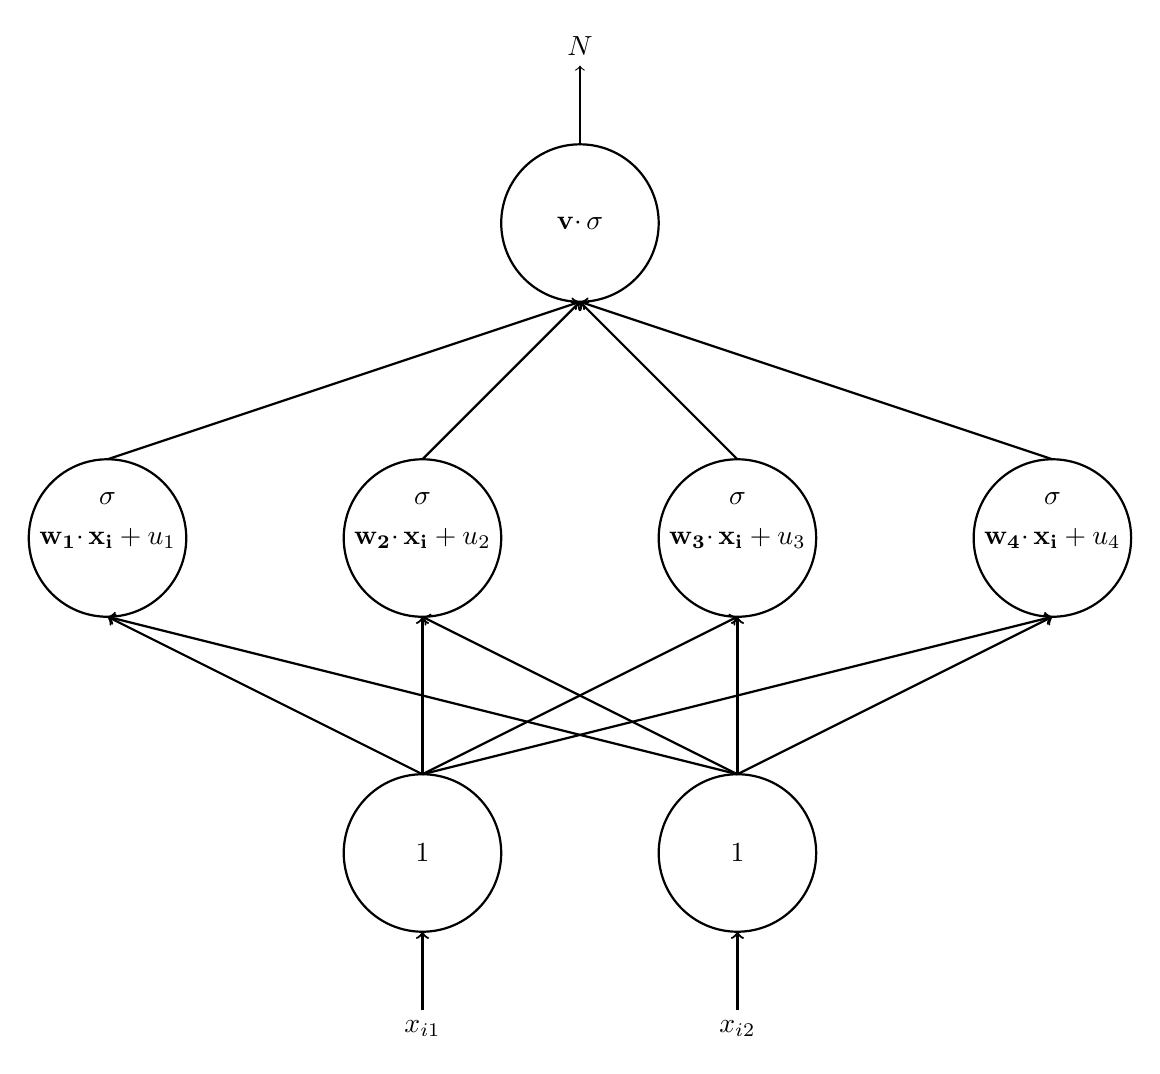
\begin{tikzpicture}

  % Input nodes
  \draw[black,thick] (0,0)  circle (1) node[anchor=center]{$1$};
  \draw[black,thick] (4,0)  circle (1) node[anchor=center]{$1$};

  % Hidden nodes
  \draw[black,thick] (-4,4) circle (1) node[anchor=center]{$\mathbf{w_1} \cdotp \mathbf{x_i} + u_1$};
  \draw[black,thick] (-4,4.5) node[anchor=center]{$\sigma$};
  \draw[black,thick] (0,4) circle  (1) node[anchor=center]{$\mathbf{w_2} \cdotp \mathbf{x_i} + u_2$};
  \draw[black,thick] (0,4.5) node[anchor=center]{$\sigma$};
  \draw[black,thick] (4,4) circle  (1) node[anchor=center]{$\mathbf{w_3} \cdotp \mathbf{x_i} + u_3$};
  \draw[black,thick] (4,4.5) node[anchor=center]{$\sigma$};
  \draw[black,thick] (8,4) circle  (1) node[anchor=center]{$\mathbf{w_4} \cdotp \mathbf{x_i} + u_4$};
  \draw[black,thick] (8,4.5) node[anchor=center]{$\sigma$};

  % Output node
  \draw[black,thick] (2,8) circle  (1) node[anchor=center]{$\mathbf{v} \cdotp \mathbf{\sigma}$};

  % Connect input nodes to hidden nodes.
  \draw[black,thick,->] (0,1) -- (-4,3);
  \draw[black,thick,->] (0,1) -- (0,3);
  \draw[black,thick,->] (0,1) -- (4,3);
  \draw[black,thick,->] (0,1) -- (8,3);
  \draw[black,thick,->] (4,1) -- (-4,3);
  \draw[black,thick,->] (4,1) -- (0,3);
  \draw[black,thick,->] (4,1) -- (4,3);
  \draw[black,thick,->] (4,1) -- (8,3);

  % Connect hidden nodes to output node.
  \draw[black,thick,->] (-4,5) -- (2,7);
  \draw[black,thick,->] (0,5) --  (2,7);
  \draw[black,thick,->] (4,5) --  (2,7);
  \draw[black,thick,->] (8,5) --  (2,7);

  % Network inputs
  \draw[black] (0,-2) node[anchor=north]{$x_{i1}$};
  \draw[black] (4,-2) node[anchor=north]{$x_{i2}$};
  \draw[black,thick,->] (0,-2) -- (0,-1);
  \draw[black,thick,->] (4,-2) -- (4,-1);

  % Network output
  \draw[black,->] (2,9) -- (2,10) node[anchor=south] {$N$};

\end{tikzpicture}
\caption{Schematic of a simple feed-forward neural network.}
\end{figure}

An example of the neural network structure used in the current work is illustrated in Figure \ref{fig:ffnn}. In a feedforward network of this type, the input signals $\mathbf x$ are sent to each hidden node via distinct connections, where they are weighted, summed, and transformed as discussed previously. The outputs from the hidden layer are then combined at the single output node in the same fashion, but without a bias, and an identity transfer function:

\begin{equation}
  N = \sum_{k=1}^H v_k \sigma_k
\end{equation}

%%%%%%%%%%%%%%%%%%%%%%%%%%%%%%%%%%%%%%%%%%%%%%%%%%%%%%%%%%%%%%%%%%%%%%%%%%%%%%%%

\newpage

\section{Methods and Techniques}

\subsection{The nnode software}

The general approach described in the previous sections has been implemented in a library of Python code called \texttt{nnode}. It has been successfully applied to a variety of simple ordinary and partial differential equations. Below are examples of use of this code to solve one- and two-dimensional diffusion problems.

Note that these problems are initial value problems in time. In such cases, the second term for the time variable is dropped in the construction of the boundary condition function.

\subsection{Examples}

\subsubsection{The Diffusion Equation}

Consider the diffusion equation ($\nabla$ is the spatial gradient operator):

\begin{equation}
  G \left( \mathbf x, \psi, \nabla \psi, \nabla^2 \psi \right) = \frac {\partial \psi} {\partial t} - D \nabla^2 \psi = 0
\end{equation}

\subsubsection{The One-Dimensional Diffusion Equation}

In one spatial dimension, this becomes (note that $\mathbf x = (x,t)$:

\begin{equation}
  G \left( \mathbf x, \psi, \nabla \psi, \nabla^2 \psi \right) = \frac {\partial \psi} {\partial t} - D \frac {\partial^2 \psi} {\partial^2 x} = 0
\end{equation}

Assume the presence of Dirichlet boundary conditions:

\begin{equation}
\begin{split}
  \psi(0,t) &= 0 \\
  \psi(1,t) &= 0 \\
  \psi(x,0) &= \sin(\pi x)
\end{split}
\end{equation}

This problem has an analytical solution (not in general true for PDEs):

\begin{equation}
  \psi_a(\mathbf x) = e^{-\pi^2 D t} \sin(\pi x)
\end{equation}

With these boundary conditions, the boundary condition function, network coefficient function, and trial function reduce to:

\begin{equation}
\begin{split}
  A(\mathbf x) &= (1 - t)\sin(\pi x) \\
  P(\mathbf x) &= x(1 - x)t \\
  \psi_t(\mathbf x,\mathbf p) &= (1 - t)\sin(\pi x) + x(1 - x)t N(\mathbf x,\mathbf p)
\end{split}
\end{equation}

A neural network was constructed using $H=10$ hidden nodes. All weights and biases were initialized with uniform random numbers in the range $[-1,1]$. A uniform $10\times10$ grid of training points in the domain $0 \leq x,t \leq 1$ was created for training. Results are shown in Figures \ref{fig:diff1d_trained} and \ref{fig:diff1d_error}. In general, the errors were of $O(10^{-5})$ or smaller.

\begin{figure}
    \centering
    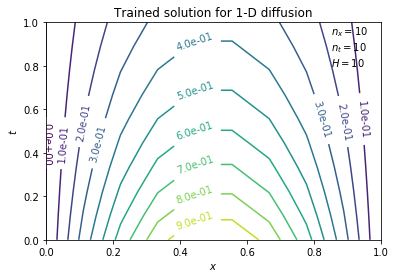
\includegraphics[width=0.5\textwidth]{figures/diff1d_trained.png}
    \caption{Trained solution for one-dimensional diffusion problem.}
    \label{fig:diff1d_trained}
\end{figure}

\begin{figure}
    \centering
    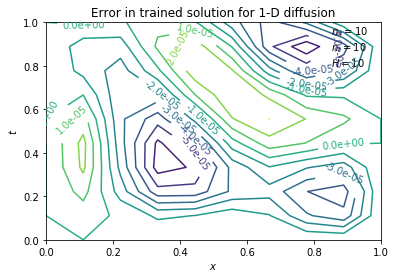
\includegraphics[width=0.5\textwidth]{figures/diff1d_error.png}
    \caption{Error in trained solution for one-dimensional diffusion problem.}
    \label{fig:diff1d_error}
\end{figure}

\subsubsection{The Two-Dimensional Diffusion Equation}

In this case, the diffusion equation may be written as:

\begin{equation}
  G \left( \mathbf x, \psi, \nabla \psi, \nabla^2 \psi \right) = \frac {\partial \psi} {\partial t} - D \left( \frac {\partial^2 \psi} {\partial^2 x} +  \frac {\partial^2 \psi} {\partial^2 y} \right) = 0
\end{equation}

Assume the presence of the following Dirichlet boundary conditions:

\begin{equation}
\begin{split}
  \psi(0,y,t) &= 0 \\
  \psi(1,y,t) &= 0 \\
  \psi(x,0,t) &= 0 \\
  \psi(x,1,t) &= 0 \\
  \psi(x,y,0) &= \sin(\pi x) \sin(\pi y)
\end{split}
\end{equation}

This problem has an analytical solution (not in general true for PDEs):

\begin{equation}
  \psi_a(\mathbf x) = e^{-2\pi^2 D t} \sin(\pi x) \sin(\pi y)
\end{equation}

With these boundary conditions, the boundary condition function, network coefficient function, and trial function reduce to:

\begin{equation}
\begin{split}
  A(\mathbf x) &= (1 - t)\sin(\pi x) \sin(\pi y) \\
  P(\mathbf x) &= x(1 - x)y(1 - y)t \\
  \psi_t(\mathbf x,\mathbf p) &= (1 - t)\sin(\pi x) \sin(\pi y) + x(1 - x)y(1 - y)t N(\mathbf x,\mathbf p)
\end{split}
\end{equation}

A neural network was constructed using $H=10$ hidden nodes. All weights and biases were initialized with uniform random numbers in the range $[-1,1]$. A uniform $10\times10\times10$ grid of training points in the domain $0 \leq x,y,t \leq 1$ was created for training. Results are shown in Figures \ref{fig:diff2d_trained} and \ref{fig:diff2d_error}. In general, the errors were of $O(10^{-3})$ or smaller. The increase in error is not surprising, since the size of the network was not increased to account for the larger problem. Even with this small network, the solution was reasonably accurate (within $O(10^{-2}$)) over the entire domain.

\begin{figure}
\centering
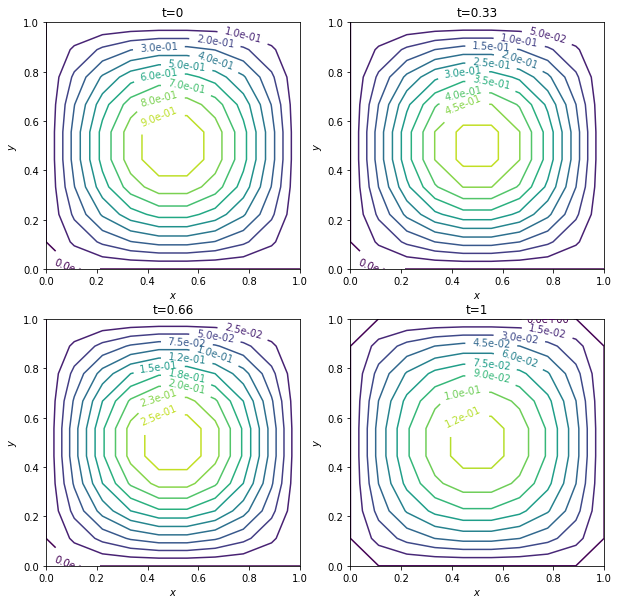
\includegraphics[width=0.5\textwidth]{figures/diff2d_trained.png}
\caption{Trained solution for two-dimensional diffusion problem.}
\label{fig:diff2d_trained}
\end{figure}

\begin{figure}
\centering
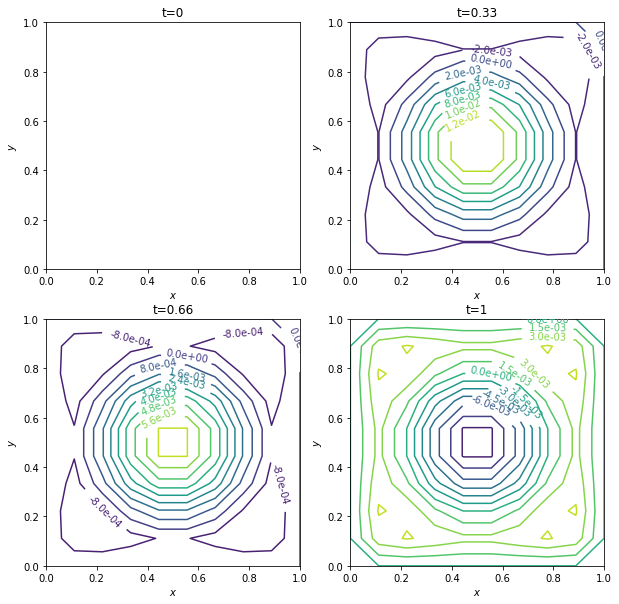
\includegraphics[width=0.5\textwidth]{figures/diff2d_error.png}
\caption{Error in trained solution for two-dimensional diffusion problem.}
\label{fig:diff2d_error}
\end{figure}

\subsubsection{The One-Dimensional Diffusion Equation With Time-Varying Boundary Conditions}

This problem is similar to the previous one-dimensional problem, but now the Dirichlet boundary condition at $x=1$ is a function of time:

\begin{equation}
\begin{split}
  \psi(0,t) &= 0 \\
  \psi(1,t) &= 0.1 t\\
  \psi(x,0) &= \sin(\pi x)
\end{split}
\end{equation}


The same network architecture and initialization procedure was used as that for the original one-dimensional diffusion example. Results are shown in Figures \ref{fig:diff1d_dynamicBC_trained} and \ref{fig:diff1d_dynamicBC_error}. The solution error is appreciable now, again since a relatively small network was used to develop the solution. Increasing the number of nodes in the hidden layer was shown to increase the accuracy of the solution.

\begin{figure}
    \centering
    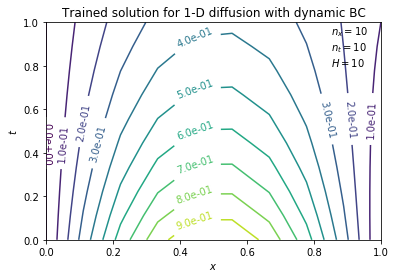
\includegraphics[width=0.5\textwidth]{figures/diff1d_dynamicBC_trained.png}
    \caption{Trained solution for one-dimensional diffusion problem with dynamic BC.}
    \label{fig:diff1d_dynamicBC_trained}
\end{figure}

\begin{figure}
    \centering
    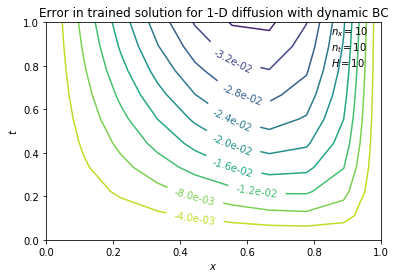
\includegraphics[width=0.5\textwidth]{figures/diff1d_dynamicBC_error.png}
    \caption{Error in trained solution for one-dimensional diffusion problem with dynamic BC.}
    \label{fig:diff1d_dynamicBC_error}
\end{figure}

\subsection{Discussion}

The examples shown above, and many others not shown, indicate that the initial version of the \texttt{nnode} software is capable of solving relatively simple partial differential equations with static and dynamic boundary conditions. In the proposed work, the code swill be further developed to handle the coupled set of partial differential equations which are the MHD equations.

%%%%%%%%%%%%%%%%%%%%%%%%%%%%%%%%%%%%%%%%%%%%%%%%%%%%%%%%%%%%%%%%%%%%%%%%%%%%%%%%

\newpage

\section{Timeline}

The existing \texttt{nnode} code will be enhanced in stages. At each stage, code will be tested using a standardized set of generic example problems, as well as the results of standard space physics models (see discussion in previous sections). These problems will include those with analytical solutions as well as those which require FDM or FEM solutions. Validation of results will be completely automated, and built into the test suite for the entire \texttt{nnode} package. Numerical solutions will be generated by 3rd-party data providers, e.g. CCMC, or computed with a standard PDE solution package, such as the NDSolve() function in Mathematica.

\subsection{Select Reference Scenarios}

Planned completion date: August 2020

In this stage, a definitive list of reference problems, both generic and space weather-specific, will be documented. Generic problems from the literature, e.g. \cite{Lagaris1998} will be used, as well as a carefully-selected set of models from the space physics community, such as the CCMC and the SWPC.

\subsection{Adapt Code to Multiprocessing System}

Planned completion date: December 2020

In this stage, the code will be upgraded to take advantage of parallel computing facilities. Initially, this work will target the science computing cluster at the Space Telescope Science Institute in Baltimore, Maryland. This first stage will involve coarse parallelization - splitting the computation among available cores on the host machines. If time permits, the code will be further upgraded to take advantage of available accelerator technology, e.g. general-purpose graphical processing (GPGPU) cards. The progress of this latter capability will be dependent upon resource availability. If needed, existing GPGPU facilities at GMU will be utilized. Completion of this step will greatly broaden the scope of problems which can be addressed by the \texttt{nnode} software. Based on past experience with parallel codes, execution speed is expected to increase by at least an order of magnitude. The core of the code may undergo a redesign at this stage, to incorporate higher-performance machine learning libraries, such as TensorFlow and PyTorch.

\subsection{Add Capability to Solve Systems of PDEs}

Planned completion date: May 2021

This will be a relatively straightforward addition to the software. The modifications will start with simple aggregation of network outputs and errors in an overarching error function, and the consequent additional level of derivatives. This approach has already been shown to work in the literature \cite{Lagaris1998}. Another possible approach is the use of vector-valued neural networks, but this approach has not been examined to date.

\subsection{Demonstrate Applicability to MHD Equations for Space Weather}

Planned completion date: August 2021

This phase constitutes the physical core of the investigation. During the prior development phases, a variety of well-understood space weather phenomena will be examined. One or more representative problems will be selected on the basis of simplicity, and the availability of real-world data against which the solution can be compared. These problems will then be used to demonstrate the real-world utility of the \texttt{nnode} software.

\subsection{Write and Present Thesis}

Planned completion date: December 2021

%%%%%%%%%%%%%%%%%%%%%%%%%%%%%%%%%%%%%%%%%%%%%%%%%%%%%%%%%%%%%%%%%%%%%%%%%%%%%%%%

\medskip

\printbibliography[heading=bibintoc]

%%%%%%%%%%%%%%%%%%%%%%%%%%%%%%%%%%%%%%%%%%%%%%%%%%%%%%%%%%%%%%%%%%%%%%%%%%%%%%%%

\end{document}